\section{ĐỊNH LÝ PYTHAGORE.}
%\subsection{Định lý Pythagore}
\subsubsection{Kiến thức trọng tâm}
\begin{tomtat}
\begin{dn}
		\textbf{Định lý Pythagore}\\
	Trong một tam giác vuông, bình phương của cạnh huyền bằng tổng các bình phương của hai cạnh góc vuông.
\end{dn}
\begin{dn}
		\textbf{Định lý Pythagore đảo}\\
	Nếu một tam giác có bình phương của một cạnh bằng tổng các bình phương của hai cạnh kia thì đó là tam giác vuông.
\end{dn}
\end{tomtat}

\begin{vd}%[Dự án EX-8-Đề Cương Toán 8]%[Nguyễn Văn Cường 056]%[8H5V1-1]
	Tính độ dài cạnh $EF$, $MN$, $AC$ của các tam giác vuông trong hình sau.
	\begin{center}
		
		\begin{tikzpicture}[scale=1,font=\footnotesize, line join=round, line cap=round, >=stealth]
			\def\r{3}
			\path
			(0,0) coordinate (O)
			(-\r,0) coordinate (E)
			(\r,0) coordinate (F)
			(130:\r) coordinate (D)
			;
			\draw 
			(D)--(E)--(F)--cycle
			pic[draw,angle radius=2mm]{right angle=E--D--F}
			;
			\path (E)--(D) node[pos=.5,sloped, rotate=0, above]{$5$ cm};
			\path (D)--(F) node[pos=.5,sloped, rotate=0, above]{$12$ cm};
			\node[below] at (0,-.5){a)};
			\foreach \x/\g in {D/90,E/-180,F/0} \fill[black] (\x) circle (1pt)+(\g:.3) node {$\x$};
		\end{tikzpicture}
		\begin{tikzpicture}[scale=1,font=\footnotesize, line join=round, line cap=round, >=stealth]
			\def\r{2}
			\path
			(0,0) coordinate (O)
			(-160:\r) coordinate (N)
			(30:\r) coordinate (P)
			(110:\r) coordinate (M)
			;
			\draw 
			(M)--(N)--(P)--cycle
			pic[draw,angle radius=2mm]{right angle=N--M--P}
			;
			\path (M)--(P) node[pos=.5,sloped, rotate=0, above]{$3$ cm};
			\path (N)--(P) node[pos=.5,sloped, rotate=0, above]{$4$ cm};
			\node[below] at (0,-1){b)};
			\foreach \x/\g in {M/90,N/-180,P/0} \fill[black] (\x) circle (1pt)+(\g:.3) node {$\x$};
		\end{tikzpicture}
\begin{tikzpicture}[line join = round, line cap = round,>=stealth,font=\footnotesize,scale=1]
\def\r{3}
\path
(0,0) coordinate (O)
(-\r,0) coordinate (O1)
(\r,0) coordinate (O2)
(140:\r) coordinate (O3)
;
\pgfresetboundingbox
\draw (O1)--(O2)--(O3) --(O1)node[midway,left]{$8$ cm}--(O2)node[midway,below]{$17$ cm};
\pic[draw, angle radius=8pt]{right angle=O1--O3--O2};
\foreach\i/\j/\k in{O1/B/180,O2/C/0,O3/A/90}
\fill[black](\i)circle(1.5pt)node[shift=(\k:2.5mm)]{$\j$};
\node[below] at (0,-.5){c)};
\end{tikzpicture}
\end{center}
\loigiai{
\begin{enumerate}
\item 	Áp dụng định lí Pythagore vào tam giác vuông $DEF$, ta có
\begin{eqnarray*}
	&&EF^2 = ED^2+DF^2\\ 
	&&EF^2=5^2+12^2\\
	&&EF^2=169\\
	&&EF=\sqrt{169}\\
	&&EF=13.
\end{eqnarray*}
Vậy $EF=13$ cm.
\item Áp dụng định lí Pythagore vào tam giác vuông $MNP$, ta có
\begin{eqnarray*}
&&	NP^2 = MN^2+MP^2\\ 
&&	MN^2=NP^2-MP^2\\
&&	MN^2=4^2-3^2\\
&&	MN^2=7\\
&&	MN=\sqrt{7}.
\end{eqnarray*}
Vậy $MN=\sqrt{7}$ cm.
\item Áp dụng định lí Pythagore vào tam giác vuông $ABC$, ta có
\begin{eqnarray*}
	&&BC^2=AB^2+AC^2\\
	&&BC^2=8^2+15^2\\
	&&BC^2=64+225\\
	&&BC^2=289\\
	&&BC=\sqrt{289}=17.
\end{eqnarray*}
Vậy $BC=17$ cm.
\end{enumerate}
}
\end{vd}
\begin{vd}%[Dự án EX-8-Đề Cương Toán 8]%[Nguyễn Văn Cường 056]%[8H5H1-3]
Chứng minh các tam giác sau vuông
	\begin{enumerate}
		\item Tam giác $ABC$ có $AB=3$ cm, $BC=5$ cm, $AC=4$ cm.
		\item Tam giác $MNP$ có $MN=20$ m, $NP=12$ m, $PM=16$ m.
	\end{enumerate}
	\loigiai{
		\begin{enumerate}
			\item Ta có $AB^2=9$; $BC^2=25$; $AC^2=16$.\\
			Suy ra $BC^2=AB^2+AC^2$.\\
			Vậy tam giác $ABC$ vuông tại $A$ (Pythagore đảo).
			\item Ta có $MN^=400$; $NP^2=144$; $PM^2=256$.\\
		Suy ra $MN^2=NP^2+PM^2$. \\
			Vậy tam giác $MNP$ vuông tại $P$ (Pythagore đảo).
		\end{enumerate}
	}	
\end{vd}
\begin{vd}%[Dự án EX-8-Đề Cương Toán 8]%[Nguyễn Văn Cường 056]%[8H5V1-4]
	Một con thuyền đang neo ở một điểm cách chân tháp hải đăng $180$ m. Biết tháp hải đăng cao $25$ m. Khoảng cách từ thuyền đến đỉnh tháp hải đăng bằng? (làm tròn kết quả đến hàng phần mười)
	\begin{center}
		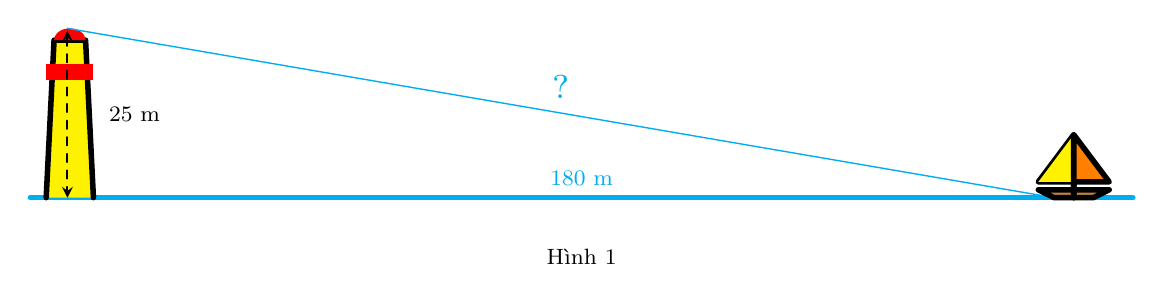
\begin{tikzpicture}[line join = round, line cap=round,>=stealth,font=\footnotesize,scale=1,line width=2pt]
			\draw[cyan] (0,0)--(14,0) node[pos=0.5,above]{$180$ m};
			\fill[yellow]  (0.2,0)--(0.3,2)--(0.7,2)--(0.8,0); %%%thân tháp
			\draw  (0.2,0)--(0.3,2)--(0.7,2)--(0.8,0); %%%thân tháp
			\fill[red] (0.3,2) arc(0:180:-0.2cm and 0.15cm)--(0.7,2)--cycle; %%%% chóp
			\fill[red] (0.2,1.5) rectangle (0.8,1.7);
			\draw[cyan,line width=0.5pt] (0.47,2.15)--(13,0) node[pos=0.5,above,scale=1.5]{?};
			\fill[brown] (13,0)--(12.8,0.1)--(13.7,0.1)--(13.5,0)--cycle;
			\draw (13,0)--(12.8,0.1)--(13.7,0.1)--(13.5,0)--cycle;
			\draw (13.25,0)--(13.25,0.8)--(12.8,0.2)--(13.25,0.2);
			\fill[yellow] (13.25,0)--(13.25,0.8)--(12.8,0.2)--(13.25,0.2);
			\fill[orange] (13.25,0)--(13.25,0.8)--(13.7,0.2)--(13.7,0.2)--(13.25,0.2);
			\draw (13.25,0)--(13.25,0.8)--(13.7,0.2)--(13.7,0.2)--(13.25,0.2);
			\draw (7,0)node[below=0.5cm]{Hình 1};
			\draw[<->,line width=0.7pt,dashed] (0.47,2.12)--(0.47,0) node[pos=0.5,right=0.4cm]{$25$ m};
		\end{tikzpicture}
	\end{center}
	\loigiai{
		Khoảng cách từ thuyền đến đỉnh tháp hải đăng là $\sqrt{180^2+25^2}\approx 181{,}7$ m.
	}
\end{vd}
\subsubsection{Bài tập}
\begin{bt}%[Dự án EX-8-Đề Cương Toán 8]%[Nguyễn Văn Cường 056]%[8H5V1-1]
	Tìm độ dài $x$ trong các tam giác vuông ở hình sau.
\begin{center}
\begin{tikzpicture}[line join = round, line cap = round,>=stealth,font=\footnotesize,scale=1]
\path (0,0) coordinate (O1) (4,0) coordinate (O2) (4,3) coordinate (O3);
\draw (O1)--(O2)node[midway,below]{$x$}--(O3)node[midway,right]{$6$}--(O1)node[midway,left]{$10$};
\pic[draw, angle radius=8pt]{right angle=O3--O2--O1};
\path ($(O1)!.5!(O2)$)node[shift=(-90:6mm)]{$a)$};
\foreach\i/\j/\k in{O1/M/180,O2/N/0,O3/I/90}
\fill[black](\i)circle(1.5pt)node[shift=(\k:2.5mm)]{$\j$};
\end{tikzpicture}
\hspace{2cm}
\begin{tikzpicture}[line join = round, line cap = round,>=stealth,font=\footnotesize,scale=1]
\path (0,0) coordinate (O1) ({2*sqrt(2)},0) coordinate (O2);
\path[name path=a] (O1) circle (2);
\path[name path=b] (O2) circle (2);
\path[name intersections={of=a and b,by={O3,O4}}];
\pgfresetboundingbox
\draw (O1)--(O2)node[midway,below]{$x$}--(O3)node[midway,right]{$1$}--(O1)node[midway,left]{$1$};
\pic[draw, angle radius=8pt]{right angle=O1--O3--O2};
\foreach\i/\j/\k in{O1/H/180,O2/G/0,O3/K/90}
\fill[black](\i)circle(1.5pt)node[shift=(\k:2.5mm)]{$\j$};
\path ($(O1)!.5!(O2)$)node[shift=(-90:6mm)]{$b)$};
\end{tikzpicture}
\hspace{2cm}
\begin{tikzpicture}[line join = round, line cap = round,>=stealth,font=\footnotesize,scale=1]
	\path (0,0) coordinate (O1) (5.4,0) coordinate (O2) (5.4,3) coordinate (O3);
	\draw (O1)--(O2)node[midway,below]{$37{,}8$}--(O3)node[midway,right]{$21$}--(O1)node[midway,above]{$x$};
	\pic[draw, angle radius=8pt]{right angle=O3--O2--O1};
	\foreach\i/\j/\k in{O1/A/180,O2/C/0,O3/B/90}
	\fill[black](\i)circle(1.5pt)node[shift=(\k:2.5mm)]{$\j$};
	\node[below] at (2,-.5){c)};
\end{tikzpicture}
\hspace{2cm}
\begin{tikzpicture}[scale=1,font=\footnotesize, line join=round, line cap=round, >=stealth]
\def\r{3}
\path
(0,0) coordinate (O)
(-\r,0) coordinate (E)
(\r,0) coordinate (F)
(130:\r) coordinate (D)
;
\draw 
(D)--(E)--(F)--cycle
pic[draw,angle radius=2mm]{right angle=E--D--F}
;
\path (E)--(D) node[pos=.5,sloped, rotate=0, above]{$10$};
\path (D)--(F) node[pos=.5,sloped, rotate=0, above]{$24$};
\path (E)--(F) node[pos=.5,sloped, rotate=0, below]{$x$};
\node[below] at (1,-.5){d)};
%	\node[below] at (3,-1.5){Hình 3};
\foreach \x/\g in {D/90,E/-180,F/0} \fill[black] (\x) circle (1pt)+(\g:.3) node {$\x$};
\end{tikzpicture}
\hspace{2cm}
\begin{tikzpicture}[scale=1,font=\footnotesize, line join=round, line cap=round, >=stealth]
\def\r{2}
\path
(0,0) coordinate (O)
(-160:\r) coordinate (N)
(30:\r) coordinate (P)
(110:\r) coordinate (M)
;
\draw 
(M)--(N)--(P)--cycle
pic[draw,angle radius=2mm]{right angle=N--M--P}
;
\path (M)--(P) node[pos=.5,sloped, rotate=0, above]{$4{,5}$};
\path (N)--(P) node[pos=.5,sloped, rotate=0, below]{$6$};
\path (N)--(M) node[pos=.5,sloped, rotate=0, above]{$x$};
\node[below] at (1.0,-1){e)};
\foreach \x/\g in {M/90,N/-180,P/0} \fill[black] (\x) circle (1pt)+(\g:.3) node {$\x$};
\end{tikzpicture}
\hspace{2cm}
\begin{tikzpicture}[line join = round, line cap = round,>=stealth,font=\footnotesize,scale=1]
\def\r{3}
\path
(0,0) coordinate (O)
(-\r,0) coordinate (O1)
(\r,0) coordinate (O2)
(140:\r) coordinate (O3)
;
\pgfresetboundingbox
\draw (O1)--(O2)--(O3)node[midway,above]{$x$} --(O1)node[midway,left]{$8$}--(O2)node[midway,below]{$17$};
\pic[draw, angle radius=8pt]{right angle=O1--O3--O2};
\foreach\i/\j/\k in{O1/B/180,O2/C/0,O3/A/90}
\fill[black](\i)circle(1.5pt)node[shift=(\k:2.5mm)]{$\j$};
\node[below] at (1,-.5){f)};
\end{tikzpicture}
\end{center}
	\loigiai{
\begin{enumerate}
\item 
Xét $\triangle MNI$ vuông tại $N$\\
Áp dụng định lý Pythagore, ta có
\begin{eqnarray*}
	&&MI^2=MN^2+NI^2\\
	&&10^2=x^2+6^2\\
	&&x^2=10^2-6^2=100-36=64.
\end{eqnarray*}
Suy ra $x=\sqrt{64}=8$.\\
Vậy $x=8$.
\item Xét $\triangle HKG$ vuông tại $K$\\
Áp dụng định lý Pythagore, ta có
\begin{eqnarray*}
	&&HG^2 = HK^2 + KG^2 \\
	&&x^2 = 1^2 + 1^2 = 2.
\end{eqnarray*}
Suy ra $x = \sqrt{2}$.\\
Vậy $x = \sqrt{2}$.
\item Xét $\triangle ABC$ vuông tại $C$\\
Áp dụng định lý Pythagore, ta có
\begin{eqnarray*}
	&&AB^2 = AC^2 + BC^2 \\
	&&x^2 = 37{,}8^2 + 21^2 \\
	&&x^2 = 1428{,}84 + 441 = 1869{,}84.
\end{eqnarray*}
Suy ra $x = \sqrt{1869{,}84} \approx 43{,}24$.\\
Vậy $x \approx 43{,}24$.
\item Xét $\triangle EDF$ vuông tại $D$\\
Áp dụng định lý Pythagore, ta có
\begin{eqnarray*}
	&&EF^2 = ED^2 + DF^2 \\
	&&x^2 =10^2 + 24^2 = 100 + 576 = 676.\\
\end{eqnarray*}
Suy ra $x = \sqrt{676} = 26$.\\
Vậy $x = 26$.
\item Xét $\triangle MNP$ vuông tại $M$\\
Áp dụng định lý Pythagore, ta có
\begin{eqnarray*}
	&&NP^2 = MN^2 + MP^2 \\
	&&6^2 = x^2 + 4{,}5^2 \\
	&&36 = x^2 + 20{,}25 \\
	&&x^2 =  36-20{,}25\\
	&&x^2 = 15{,}75.
\end{eqnarray*}
Suy ra $x = \sqrt{15{,}75} \approx 3{,}97$.\\
Vậy $x \approx 3{,}97$.
\item Xét $\triangle ABC$ vuông tại $A$\\
Áp dụng định lý Pythagore, ta có
\begin{eqnarray*}
	&&BC^2 = AB^2 + AC^2 \\
	&&17^2 = 8^2 + x^2 \\
	&&289 = 64 + x^2 \\
	&&x^2 = 289-64\\
	&&x^2 = 225.
\end{eqnarray*}
Suy ra $x = \sqrt{225} = 15$.\\
Vậy $x = 15$.\\
\end{enumerate}
	}
\end{bt}
\begin{bt}%[Dự án EX-8-Đề Cương Toán 8]%[Nguyễn Văn Cường 056]%[8H5H1-3]
	Chứng minh các tam giác sau là tam giác vuông.
	\begin{enumerate}
		\item Tam giác $ABC$ có $AB = 6$ cm, $BC = 8$ cm, $AC = 10$ cm.
		\item Tam giác $DEF$ có $DE = 5$ cm, $EF = 13$ cm, $FD = 12$ cm.
		\item Tam giác $GHI$ có $GH = 9$ cm, $HI = 12$ cm, $IG = 15$ cm.
		\item Tam giác $JKL$ có $JK = 7$ cm, $KL = 24$ cm, $LJ = 25$  cm.
		\item Tam giác $MNO$ có $MN = 8$ cm, $NO = 15$ cm, $OM = 17$ cm.
		\item Tam giác $PQR$ có $PQ = 10$ cm, $QR = 24$ cm, $RP = 26$ cm.
	\end{enumerate}
	\loigiai{
		\begin{itemize}
			\item $AB^2+BC^2=6^2+8^2=36+64=100=10^2=AC^2$ .\\ Suy ra $ \triangle ABC$ vuông tại $B$ (Theo định lý Pythagore). 
			\item  $DE^2+DF^2=5^2+12^2=25+144=169=13^2=EF^2$ .\\ Suy ra $ \triangle DEF$ vuông tại $D$ (Theo định lý Pythagore).
			\item  $GH^2+HI^2=9^2+12^2=81+144=225=15^2=IG^2$ .\\ Suy ra $ \triangle GHI$ vuông tại $H$ (Theo định lý Pythagore).
			\item  $JK^2+KL^2=7^2+24^2=49+576=625=25^2=LJ^2$ .\\ Suy ra $ \triangle JKL$ vuông tại $K$ (Theo định lý Pythagore).
			\item $MN^2+NO^2=8^2+15^2=64+225=289=17^2=OM^2$ .\\ Suy ra $ \triangle MNO$ vuông tại $N$ (Theo định lý Pythagore).
			\item $PQ^2+QR^2=10^2+24^2=100+576=676=26^2=RP^2$ .\\ Suy ra $ \triangle PQR$ vuông tại $Q$ (Theo định lý Pythagore).
		\end{itemize}
	}
\end{bt}
\begin{bt}%[Dự án EX-8-Đề Cương Toán 8]%[Nguyễn Văn Cường 056]%[8H5H1-3]
	Kiểm tra xem các tam giác sau có phải là tam giác vuông hay không?
	\begin{enumerate}
		\item Tam giác $ABC$ có $AB = 7$, $BC = 24$, $AC = 25$ m.
		\item Tam giác $DEF$ có $DE = 6$, $EF = 10$, $FD = 8$ cm.
		\item Tam giác $GHI$ có $GH = 5$, $HI = 7$, $IG = 9$ cm.
		\item Tam giác $JKL$ có $JK = 9$, $KL = 40$, $LJ = 41$ m.
		\item Tam giác $MNO$ có $MN = 13$, $NO = 14$, $OM = 15$ cm.
		\item Tam giác $PQR$ có $PQ = 8$, $QR = 15$, $RP = 17$ m.
	\end{enumerate}
	\loigiai{
		\begin{itemize}
			\item $7^2+24^2=49+576=625=25^2$ .\\ Suy ra $ \triangle ABC$ vuông tại $B$ (Theo định lý Pythagore).
			\item $6^2+8^2=36+64=100=10^2$ .\\ Suy ra $ \triangle DEF$ vuông tại $D$ (Theo định lý Pythagore).
			\item  $5^2+7^2=25+49=74 \neq 9^2=81$ .\\ Suy ra $ \triangle GHI$ \textbf{không vuông} (Theo định lý Pythagore).
			\item $9^2+40^2=81+1600=1681=41^2$ .\\ Suy ra $ \triangle JKL$ vuông tại $K$ (Theo định lý Pythagore).
			\item $13^2+14^2=169+196=365 \neq 15^2=225$ .\\ Suy ra $ \triangle MNO$ \textbf{không vuông} (Theo định lý Pythagore).
			\item $8^2+15^2=64+225=289=17^2$ .\\ Suy ra $ \triangle PQR$ vuông tại $Q$ (Theo định lý Pythagore).
		\end{itemize}
	}
\end{bt}
\begin{bt}%[Dự án EX-8-Đề Cương Toán 8]%[Nguyễn Văn Cường 056]%[8H5V1-4]
	Cho tam giác $ABC$ vuông tại $A$ có $AB=6$ cm, $AC=8$ cm. Hãy tính độ dài cạnh $BC$, đường cao $AH$ và các đoạn thẳng $BH$ , $CH$.
	\loigiai{
		\immini{
			Áp dụng định lí Pythagore cho tam giác vuông $ABC$, ta được\\
			\allowdisplaybreaks
			\begin{eqnarray*}
				&&BC^2=AB^2+AC^2\\
				&&BC^2=6^2+8^2\\
				&&BC^2=100\\
				&&BC=\sqrt{100}.
			\end{eqnarray*}
			Vậy $BC=10$ cm.\\
			Vì diện tích của tam giác $ABC$ bằng $\dfrac{AB\cdot AC}{2}$ và cũng bằng 
			$\dfrac{AH\cdot BC}{2}$ \\
			nên $\dfrac{AB\cdot AC}{2}=\dfrac{AH\cdot BC}{2}$ hay $AH=\dfrac{AB\cdot 
				AC}{BC}=\dfrac{6\cdot8}{10}=4{,}8$ cm.\\
			Áp dụng định lí Pythagore cho tam giác vuông $AHB$, ta được\\
		\begin{eqnarray*}
	&&AB^2=AH^2+HB^2\\
	&&6^2=4{,}8^2+HB^2\\
	&&BH^2=6^2-4{,}8^2\\
	&&BH^2= 12{,}96\\
	&&BH=\sqrt{12{,}96}\\
	&&BH= 3{,}6.
\end{eqnarray*}			
		Vậy $BH=3{,}6$ cm.\\
Suy ra $CH=BC-BH=10-3{,}6=6{,}4$ cm.
		}
		{
			\begin{tikzpicture}[scale=0.9, font=\footnotesize, line join=round, line 
				cap=round, >=stealth]
				\path (0,0) coordinate (A)
				($(A)+(0:3)$) coordinate (B)
				($(A)+(90:4)$) coordinate (C)
				($(B)!(A)!(C)$) coordinate (H)
				;
				\draw (B)--(A) node[midway,below]{$6$} 
				(A)--(C) node[midway,left]{$8$} (B)--(C) (A)--(H)
				(1.5,-.75) ;
				\foreach \x/\y/\z in{C/A/B,A/H/B}
				\path pic[draw=black,angle radius = 6] {right angle = \x--\y--\z} ;	
				\foreach \d/\g in {A/225, B/-45, C/90,H/50}
				\path[draw=black,fill=white] (\d) circle(1pt) + (\g:9pt) node 
				{$\d$};	
			\end{tikzpicture}
		}
	}
\end{bt}
\begin{bt}%[Dự án EX-8-Đề Cương Toán 8]%[Nguyễn Văn Cường 056]%[8H5V1-4]
	\immini{
		Hình vẽ bên mô tả một cánh buồm có dạng tam giác vuông, được buộc vào cột buồm thẳng đứng với độ dài hai cạnh góc vuông là $12$ m và $5$ m. Tính chu vi và diện tích của cánh buồm đó.
	}{
		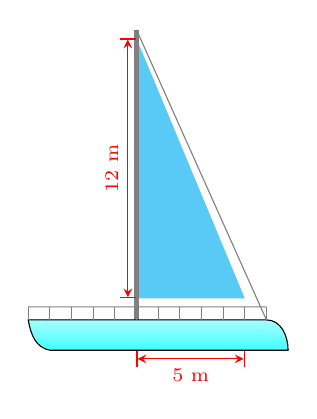
\begin{tikzpicture}[>=stealth,font=\footnotesize,scale=0.55]
			\fill[cyan!65] (0,0)--(2.5,0)--(0,6)--cycle;
			\draw[line width=1.5pt,gray] (0,-0.5)--(0,6.2);
			\fill[draw,top color=cyan!35,bottom color=cyan!75] (-2.5,-0.5) to[out=-80,in=170] (-2,-1.2)--(3.5,-1.2) to[out=90,in=0] (3,-0.5)--cycle;
			\draw[|<->|,red] (-0.2,0)--(-0.2,6)node[midway,sloped,above]{\scriptsize 12 m};
			\draw[|<->|,red] (0,-1.4)--(2.5,-1.4)node[midway,sloped,below]{\scriptsize 5 m};
			\draw[gray] (0,6.2)--(3,-0.5) (-2.5,-0.2)--(3,-0.2);
			\foreach \x in {-2.5,-2,...,3}{\draw[gray] (\x,-0.5)--++(90:0.3);}
			%	\path (current bounding box.south) node[below=2mm]	{Hình 8};
		\end{tikzpicture}
	}
	\loigiai{
		Do cánh buồm có dạng tam giác vuông với độ dài hai cạnh góc vuông là $12$ m và $5$ m nên theo định lí Pythagore ta có
		\begin{itemize}
			\item Độ dài cạnh huyền của cánh buồm đó là 
			$\sqrt{12^2+5^2}=13$ (m).
			\item Chu vi của cánh buồm là $12+5+13=30$ m.
			\item Diện tích của cánh buồm là $\dfrac{5\cdot 12}{2}=30$ m$^2$.
		\end{itemize}
	}
\end{bt}
\begin{bt}%[Dự án EX-8-Đề Cương Toán 8]%[Nguyễn Văn Cường 056]%[8H5V1-4]
	\immini{
		Hình bên mô tả mặt cắt đứng của một sân khấu ngoài trời có mái che. Chiều cao của khung phía trước khoảng $7$ m, chiều cao của khung phía sau là $6$ m, hai khung cách nhau một khoảng $5$ m. Chiều dài mái che sân khấu đó là bao nhiêu mét (làm tròn kết quả đến hàng phần trăm)?
	}{
		\begin{tikzpicture}[>=stealth,font=\footnotesize,scale=0.55]
			\fill[blue!75,draw] (0.2,0) rectangle (5.2,1.5);
			\foreach \y in {0,1,...,6}{\draw[blue!75] (0,\y)--(0.2,{\y+1})--(0,{\y+1})--(0.2,\y);}
			\foreach \y in {0,1,...,5}{\draw[blue!75] (5.2,\y)--(5.4,{\y+1})--(5.2,{\y+1})--(5.4,\y);}
			\draw[blue!75] (0,0) rectangle (0.2,7) (5.2,0) rectangle (5.4,6) (0.2,7)--(5.2,6);
			\draw[|<->|,red] (-0.3,0)--(-0.3,7)node[midway,sloped,above]{\scriptsize 7 m};
			\draw[|<->|,red] (5.7,6)--(5.7,0)node[midway,sloped,above]{\scriptsize 6 m};
			\draw[|<->|,red] (0.2,-0.3)--(5.2,-0.3)node[midway,sloped,below]{\scriptsize 5 m};
			\draw[|<->|,red] ($(0.2,7)+(70:0.3)$)--($(5.2,6)+(70:0.3)$)node[midway,sloped,above]{\scriptsize ?};
			%	\path (current bounding box.south) node[below=2mm]	{Hình 10};
		\end{tikzpicture}
	}
	\loigiai{
		\begin{center}
			\begin{tikzpicture}[>=stealth,font=\footnotesize,scale=0.55]
\path
(0,0) coordinate (O)
(5,0) coordinate (O1)
(5,6) coordinate (O2)
(0,7) coordinate (O3)
(0,6) coordinate (O4)
;
\draw (O)--(O1)--(O2)--(O3)--(O) (O2)--(O4);
			\draw[|<->|,red] (-0.3,0)--(-0.3,7)node[midway,sloped,above]{\scriptsize 7 m};
			\draw[|<->|,red] (5.7,6)--(5.7,0)node[midway,sloped,above]{\scriptsize 6 m};
			\draw[|<->|,red] (0.2,-0.3)--(5.2,-0.3)node[midway,sloped,below]{\scriptsize 5 m};
			\draw[|<->|,red] ($(0.2,7)+(70:0.3)$)--($(5.2,6)+(70:0.3)$)node[midway,sloped,above]{\scriptsize ?};
\foreach\i/\j/\k in{O2/C/70,O3/B/90,O4/A/180}
\fill[black](\i)circle(1.5pt)node[shift=(\k:4mm)]{$\j$};
		\end{tikzpicture}
		\end{center}
		Tam giác $ABC$ vuông tại $A$ có $AB=5$ m, $AC=1$ m.\\
		Theo định lí Pythagore ta có
		\[BC^2=AB^2+AC^2=5^2+1^2=26. \]
		$ BC=\sqrt{26}\approx 5{,}10$ m.\\
		Vậy chiều dài mái che sân khấu đó là $5{,}10$ m.
	}
\end{bt}
\begin{bt}%[Dự án EX-8-Đề Cương Toán 8]%[Nguyễn Văn Cường 056]%[8H5V1-4]
	\immini{
		Hình bên mô tả một thanh gỗ dài $3{,}5$ m dựa vào bức tường thẳng đứng. Chân thanh gỗ cách bức tường một khoảng là $2{,}1$ m. Khoảng cách từ điểm thanh gỗ chạm vào bức tường đến mặt đất là bao nhiêu mét?
	}{
		\begin{tikzpicture}[>=stealth,font=\footnotesize,scale=1]
			\fill[draw=orange,pattern=checkerboard,pattern color=orange] (0,0) rectangle (0.4,3.2);
			\draw[line width=2pt] (0.4,0)--(-3,0) (-2.1,0)--(0,2.8);
			\draw[line width=4pt] ($(-2.1,0)+(145:0.13)$)--($(0,2.8)+(145:0.13)$);
			\draw[|<->|,red] ($(-2.1,0)+(145:0.4)$)--($(0,2.8)+(145:0.4)$)node[midway,sloped,above]{\scriptsize 3,5 m};
			\draw[|<->|,red] (0,-0.3)--(-2.1,-0.3)node[midway,sloped,below]{\scriptsize 2,1 m};
			\draw[|<->|,red] (0.6,0)--(0.6,2.8)node[midway,right]{\scriptsize ?};
			%	\path (current bounding box.south) node[below=2mm]	{Hình 9};
		\end{tikzpicture}
	}
	\loigiai{
		\begin{center}
			\begin{tikzpicture}[line join = round, line cap = round,>=stealth,font=\footnotesize,scale=1]
	\path
	(0,0) coordinate (O)
	(-3,0) coordinate (O1)
	(90:4) coordinate (O2)
	;
	\draw (O)--(O1)--(O2)--(O);
	\pic[draw, angle radius=8pt]{right angle=O1--O--O2};
	\foreach\i/\j/\k in{O1/B/-90,O2/C/90,O/A/-90}
	\fill[black](\i)circle(1.5pt)node[shift=(\k:2.5mm)]{$\j$};
			\end{tikzpicture}
		\end{center}
		Tam giác $ABC$ vuông tại $A$ có $AB=2{,}1$ m, $BC=3{,}5$ m.\\
		Theo định lí Pythagore ta có\\
		\allowdisplaybreaks
		\begin{eqnarray*}
			&&BC^2=AB^2+AC^2\\
			&&AC^2=BC^2-AB^2\\
			&&AC^2=\left(3{,}5\right)^2-\left(2{,}1\right)^2\\
			&&AC^2= 7{,}84\\
			&&AC= 2{,}8.
		\end{eqnarray*}
		Vậy khoảng cách từ điểm thanh gỗ chạm vào bức tường đến mặt đất là $2{,}8$ m.
	}
\end{bt}
\begin{bt}%[Dự án EX-8-Đề Cương Toán 8]%[Nguyễn Văn Cường 056]%[8H5V1-4]
	\immini{
		Chú cún bị xích bởi một sợi dây dài $6$ m để canh một mảnh vườn giới hạn bởi các điểm $A$, $B$, $E$, $F$, $D$ trong hình vuông $ABCD$ có cạnh $5$ m như hình bên. Đầu xích buộc cổ cố định tại điểm $A$ của mảnh vườn. Hỏi chú cún có thể chạy đến tất cả các điểm của mảnh vườn mình phải canh không?}
	{\begin{tikzpicture}[scale=1, font=\footnotesize, line join=round, line 
			cap=round, >=stealth]
			\def\kc{3}
			%	\draw[line width=0.1mm, color=gray!50, xstep=0.1, ystep=0.1] (-.51,-.51) 
			%	grid (\kc+.4,\kc+.4);
			\draw (0,\kc)coordinate(A)--(\kc,\kc)coordinate(D)--
			(\kc,0)coordinate(C)--(0,0)coordinate(B)--cycle;
			\path ($(C)!2/5!(B)$) coordinate (E)
			($(C)!1/5!(D)$) coordinate (F)
			;
			\draw (E)--(F)--(C)node[midway,right]{$1$ m}-- 
			(C)--(E)node[midway,below]{$2$m}--(B)node[midway,below]{$3$ 
				m}(F)--(D)node[midway,right]{$4$ m};
			%	\path ($(B)!.5!(D)$) node [scale=5,xscale=-1]{\twemoji{1f415}};
			\draw(A) .. controls (.2,3) and (.6,3) ..
			(.5,2.8) .. controls (.5,2.7) and (0,2.7) ..
			(.1,2.4) .. controls (.2,2.3) and (.8,2.8) ..
			(1,2.5) .. controls (1,2.4) and (.7,2.3) ..
			(.5,2) .. controls (.5,1.9) and (.6,1.8) ..
			(1.57,1.7);
			\draw [ultra thick](1.57,1.7)--(1.8,1.65);
			\foreach \d/\g in {A/135, B/-135, C/-45,D/45,E/-90,F/0}	
			\path[draw,fill=white] (\d) circle(1pt) + (\g:8pt) node {$\d$};
		\end{tikzpicture}
	}
	\loigiai{
		$\triangle ABE$ vuông tại $B$ có
		\begin{eqnarray*}
			&&AE^2 =AB^2 +BE^2 \,\text{(định lý Pythagore)}\\
			 &&AE^2 =3^2+5^2\\
			 &&AE^2=34\\
			 &&AE=\sqrt{34}\approx 5{,}8.
		\end{eqnarray*}	
		$\triangle ADF$ vuông tại $D$ có
		\begin{eqnarray*}
			&&AF^2 =AD^2 +DF^2 \,\text{(định lý Pythagore)}\\
			 &&AE^2 =4^2+5^2\\
			 &&AE^2=41\\
			 &&AE=\sqrt{41}\approx6{,}4.
		\end{eqnarray*}	
		Vì $6{,}4$ m > $6$ m nên chú chó không đến được điểm $F$.
	}
\end{bt}
\begin{bt}%[Dự án EX-8-Đề Cương Toán 8]%[Nguyễn Văn Cường 056]%[8H5V1-4]
	Lúc $8$ giờ, một ca nô xuất phát từ một nhà giàn và chuyển động thẳng theo hướng Đông với vận tốc $24$ km/h. Cùng lúc đó, một tàu thuỷ rời nhà giàn và chuyển động thẳng theo hướng Nam với vận tốc $32$ km/h. Tính khoảng cách giữa ca nô và tàu thuỷ lúc $8$ giờ $30$ phút.
	\loigiai
	{
		\begin{center}
			\begin{tikzpicture}[line join = round, line cap = round,>=stealth,font=\footnotesize,scale=1]
				\draw[->] (0,0)--(2,0)node[right]{Đông};
				\draw[->] (0,0)--(-2,0)node[left]{Tây};
				\draw[->] (0,0)--(0,2)node[above]{Bắc};
				\draw[->] (0,0)--(0,-2)node[below]{Nam};
				\path (4,-1.3) coordinate (C) (4,2) coordinate (A) (6,2) coordinate (B);
				\foreach\i/\j in{C/180,A/135,B/90}
				\fill[black](\i)circle(1.5pt)node[shift=(\j:2.5mm)]{$\i$};
				\pic[draw, angle radius=8pt]{right angle=C--A--B};
				\draw[->] (A)--($(A)!1.2!(C)$)node[below]{Nam};
				\draw[->] (A)--($(A)!1.6!(B)$)node[right]{Đông};
				\path (C)--(B);
			\end{tikzpicture}
		\end{center}
		Gọi $A$ là vị trí của nhà giàn.\\
		Gọi $B$, $C$ lần lượt là vị trí của ca nô và tàu thuỷ lúc $8$ giờ $30$ phút.\\
		$8$ giờ $30$ phút $-$ $8$ giờ $=30$ phút $=\dfrac{1}{2}$ giờ.\\
		Quãng đường ca nô đã đi được đến $8$ giờ $30$ phút $AB=24 \cdot \dfrac{1}{2}=12$ (km).\\
		Quãng dường tàu thuỷ đã đi được đến $8$ giờ $30$ phút $AC=32 \cdot \dfrac{1}{2}=16$ (km).\\
		Ca nô và tàu thuỷ chuyển động theo hai hướng vuông góc nhau nên $\triangle ABC$ vuông
		tại $A$.\\
		\begin{eqnarray*}
			&&B C^2=A B^2+A C^2\,\text{định lý Pythagore}\\
			&&B C^2=12^2+16^2=144+256=400.
		\end{eqnarray*}
		Suy ra $BC=\sqrt{400}=20$ km.\\
		Vậy khoảng cách giữa ca nô và tàu thuỷ khi đó là $20$ km.
	}
\end{bt}